\documentclass[a4paper]{article}

\usepackage[english]{babel}
\usepackage[utf8]{inputenc}
\usepackage{amsmath}
\usepackage{minted}
\usepackage{graphicx}

\usepackage[colorinlistoftodos]{todonotes}

\title{DNS Cache Poisoning Attack}

\author{Federica Consoli - 1538420}

\date{\today}

\begin{document}
\maketitle

\begin{abstract}
	The goal of the assignment was to simulate a DNS Cache Poisoning attack. In this report I will discuss the steps taken to prepare for the hack, how it was implemented and what results were obtained.
\end{abstract}

\section{Getting started}
\label{sec:q1}
	The idea behind this hack is to make the DNS accept a specially forged packet. By design, a DNS accepts a response packet only if it matches one of its pending queries. For this to happen, the following conditions need to be satisfied:
	\begin{itemize}
		\item the response arrives on the same UDP port it was sent from
		\item the response's query ID matches the one of the pending query
		\item the response's question section matches the one of the pending query
	\end{itemize}
	The first step is, of course, to obtain the query id and the source port from the DNS server.
	\\\\
	In order to obtain these two information, I decided to use two sockets: one to query the DNS server and one to obtain its answer. The first sockets connects to the IP address of the DNS server on port 53, while the second one is listening on the same port, only this time on my machine. \\I then crafted a query packet for the DNS, asking it to lookup the address for \textit{badguy.ru} (which corresponds to my machine's address), and sent it to the DNS server via the first socket: within milliseconds, I received the information I needed on the second socket.\\
	\begin{figure}
		\centering
		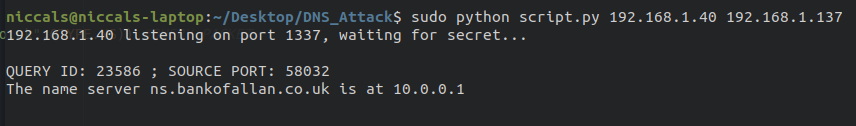
\includegraphics[width=0.9\linewidth]{qid_srcport}
		\caption[]{First steps}
		\label{fig:qidsrcport}
	\end{figure}
	\\Using a similar approach, I queried the DNS server for the IP address of the name server responsible for the victim's domain. This step is necessary because the source ip for the forged DNS responses needs to be spoofed, or else the response would not be accepted by the DNS, since it is not coming from an authoritative server for the targeted domain.
	Once I obtained the IP address, I added it as a static address for one of my machine's interfaces using the command \mintinline{bash}{ip addr add 10.0.0.1 dev lo}, which later allowed me to perform the spoofing.
\section{The program}

	





\end{document}